\documentclass[11pt]{article}

\usepackage[latin1]{inputenc}
\usepackage[T1]{fontenc}
\usepackage[french]{babel}

\usepackage{graphicx}

\addto\captionsfrench{\def\tablename{Tableau}}
\addto\captionsfrench{\def\figurename{Graphique}}

\usepackage{geometry}
\geometry{letterpaper, margin=1in}

\usepackage{url}

\begin{document}

\thispagestyle{empty}

\begin{center}

\vspace{3cm}

\textsc{\Large �cole d'actuariat}\\
\textsc{\Large Universit� Laval}\\[0.5cm]

\vspace{5cm}

{ \LARGE \bfseries Gabarit \LaTeX \\ }

\vfill

\Large Marie-Pier \textsc{C�t�}\\
{\Large \textsc{Automne} 2018}

\end{center}


\newpage

\tableofcontents

\newpage

\section{Introduction}

Dans la section~\ref{sec:commandes}, on pr�sente quelques commandes utiles, puis, des exemples de graphiques et tableaux sont donn�s dans les sections \ref{sec:graph} et \ref{sec:tab}, respectivement.

\section{Quelques commandes utiles} 
\label{sec:commandes}

Les num�ros de section et de sous-section se copieront directement dans la table des mati�res si on utilise la bonne commande. On peut r�f�rer aux sous-sections en leur assignant une �tiquette, comme � la sous-section~\ref{ssec:listes}

\subsection{Listes et �num�rations}
\label{ssec:listes}

On peut faire une �num�ration avec l'environnement suivant:

\begin{enumerate}
\item ceci est le premier point,

\item deuxi�me point, etc.
\end{enumerate}

\bigskip\noindent
Voici une autre liste:

\begin{itemize}
\item [a.] ceci est le premier point,

\item [b.] deuxi�me point, etc.
\end{itemize}

\subsection{Code}

On peut �crire du code avec l'environnement suivant:
\begin{verbatim}
n <- 1000
y <- rnorm(n)
\end{verbatim}
ou simplement utiliser \texttt{rnorm(n)}. Pour rouler \textsf{R} directement dans \LaTeX, il faut utiliser \texttt{knitr}, voir \url{https://yihui.name/knitr/}.


\subsection{�quations}

Dans le texte, on �crit les symboles math�matiques comme $\theta$. Si on veut mettre une �quation en valeur, par exemple pour $j\in \{1,\ldots, n\}$, on a
$$
Y_j= \beta_0 +\beta_1 x_j +\varepsilon_j.
$$
On peut aussi �crire
\begin{equation}\label{eq1}
s^2 = \frac{1}{n-2} \sum_{i=1}^n \hat{\varepsilon}_i^2
\end{equation}
pour pouvoir r�f�rer � l'�quation \ref{eq1} dans le texte. On ne num�rote que les �quations qui sont utilis�es.



\section{Graphiques}
\label{sec:graph}

Le graphique \ref{figure1} est enregistr� dans le dossier Figures, qui doit �tre dans le m�me dossier que le fichier source.

\begin{figure}[t!] % h = here pour ici, b = bottom pour bas de page, t = top pour haut de page
\centering
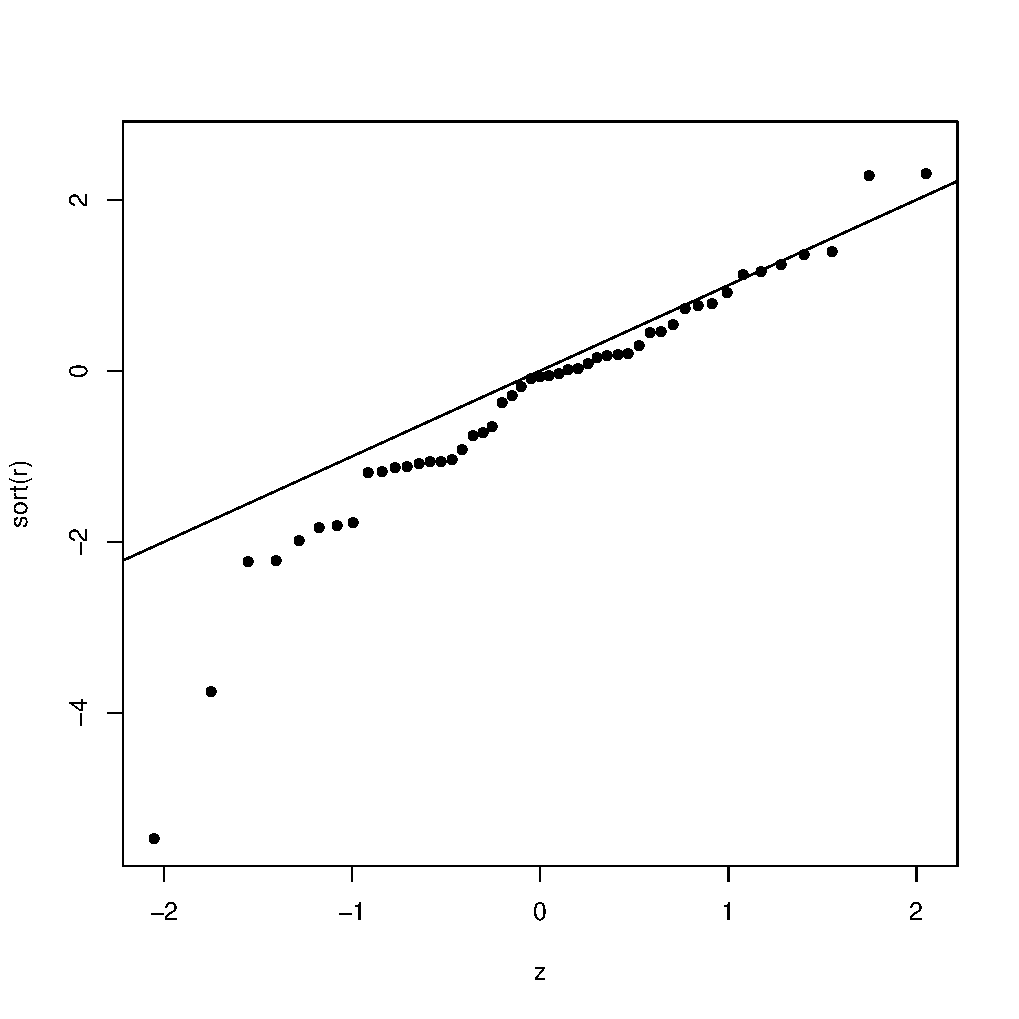
\includegraphics[width=0.5\textwidth]{Figures/Graphique.pdf}
\caption{Titre du graphique. \label{figure1}}
\end{figure}


\section{Tableaux}
\label{sec:tab}

Le tableau~\ref{tableau1} est ici.

\begin{table}[h!]

\centering

\caption{Tableau d'analyse de la variance dans le cas de la r�gression lin�aire simple.\label{tableau1}}

\medskip
\begin{tabular}{|l|cccc|}\hline
Source & Degr�s de libert� & Somme des carr�s & Carr�s moyens & $F$ \\ \hline
Mod�le & $1$ & $SSR$ & $MSR$  & $MSR/MSE$ \\ \hline
Erreur & $n-2$ & $SSE$ & $MSE$ & \\ \hline
Totale & $n-1$ & $SST$ &  & \\ \hline
\end{tabular}

\end{table}

\section{Conclusion}

Il manque certainement beaucoup de d�tails, mais je manque de temps. Amusez-vous bien.

\appendix

\section{Annexe}

Voici une annexe.

\end{document} 
